\graphicspath{{figures/chapter-oxygen/}}
% Specifies the directory where pictures are stored

\chapter{Relationship between age and oxygen}
\label{cha:oxygen}

\section{Introduction}
Characterizing the ventilation of the ocean interior is a fundamental goal of
oceanography. In order to do so, signatures of biological activity and transient
(i.e. a tracer with time-varying sources or sinks) tracers such as Chlorofluorocarbons
(CFCs) are used in to infer ventilation. The goal of this work is to evaluate
what we can learn from measurements of transient tracers and oxygen that have been
made in recent decades, focusing on the relationship between oxygen utilization
and water age inferred from transient tracers.

When examining the relationship between age and oxygen, it is generally assumed
that the two follow a negative relationship. Oxygen concentration is set at the
surface and generally decreases in the ocean interior due to biological
consumption. Age on the other hand, is set to zero at the surface and increases
in the ocean interior, characterizing the time spent since last in contact with
the surface. This relationship between age and oxygen is exploited in the
oceanography in two ways. The first is that allows for the indirect measurement
of the oxygen utilization rate to diagnose changes in ocean productivity, and
the second is that it allows for the possibility to use oxygen as a proxy for
age when examining changes in ocean circulation.

The primary sink of oxygen is the utilization by biology. For this reason, the
oxygen utilization rate (OUR) is a powerful tool for understanding ocean biology
and biogeochemistry. In the ocean interior, the OUR is generally very small and
therefore very difficult to directly measure. A commonly used solution to this is
to estimate the OUR as the derivative of the change in Apparent Oxygen Utilization
(AOU) over the change in age:

\begin{equation}
  OUR = \frac{dAOU}{d\Gamma} = \frac{d([O_{2 sat}] - [O_2])}{d\Gamma}
\end{equation}

This definition of OUR is fairly ubiquitous in the ocean biogeochemistry
community. It is referenced in multiple textbooks~\citep{Sarmiento2006,Emerson2008},
and has been used extensively in the literature to draw conclusions on organic
matter transport from the surface ocean to the deep~\citep{Jenkins}, and quantify
biological productivity in the ocean~\citep{Burd2010}. However, as discussed
in~\citet{Koeve2016}, this method for determining OUR assumes that the advective
and diffusive transports impact the age and oxygen in the same way. This will
only be strictly true if the two tracer fields have the same distribution of
internal sinks, something which in general is not the case. The authors found
that when averaged over three coupled physical and biogeochemical ocean models,
the OUR determined by this method underestimated the actual modeled OUR by a
factor of 3. This result suggests that the relationship between age and oxygen
is not as straightforward as often assumed.

Another way that oxygen and age have been combined in the field is through the
suggestion that oxygen could be used as a proxy for age for quantifying changes
in ocean circulation. While transient tracers are a useful tool for understanding
ocean circulation, there are some well-documented complications in estimating age
from such tracers~\citep{Haine2002}. Additionally, transient tracer
measurements are made much less frequently than oxygen measurements, making it
impossible to directly estimate ocean age from the historical record. To resolve
these problems, the possibility of exploiting the age-oxygen relationship and
using oxygen as a proxy for age has been suggested in the physical oceanography
community. Changes in oxygen concentration could be used to diagnose changes in
ocean circulation when age measurements are unavailable~\citep{Deutsch2005,Kwon2016}.
Similarly, \citet{Brennan2008} use AOU to improve the detectability of anthropogenic
changes in overturning in a climate model. However, in order for these methodologies
to be successful, the negative correlation relationship between age and oxygen
(or positive correlation relationship between age and AOU) would need to be robust
over time and space.

In this chapter, we evaluate the relationship between age and oxygen to shed
light on where it may be valid to use oxygen as a proxy for age and to consider
the use of defining OUR as AOU divided by mean age. Because it crosses the western
boundary current in the North Atlantic Ocean, and has measured both transient
tracer and oxygen concentrations, Line W provides a unique opportunity to
investigate the assumed negative relationship between age and oxygen and examine
the robustness of the two mentioned applications of this age-oxygen relationship.
Because of the limited temporal resolution and spatial coverage of the Line W
observational data, we seek to put the observational data in context by performing
a similar analysis of an earth system model, GFDL ESM2Mc.

In the next section we introduce the Line W observational data set, describe how
transient tracer ages were derived, and discuss the earth system model specifications.
In Section~\ref{section:results} we explore the age-oxygen relationship in the observations and model,
and discuss mechanisms driving the resulting relationship. Finally, in Section~\ref{section:conclusions}
we share our conclusions.

% METHODS


\section{Methods}
\label{section:methods}
\subsection{Line W Observational Data}
\subsubsection{Data Collection}
The observational data set used in this analysis comes from the Woods Hole Oceanographic
Institute's (WHOI) Line W ship-based repeat hydrography study~\citep{Andres2017}.
Observations include full-depth temperature and salinity profiles, horizontal
velocity profiles from lowered ADCPs (LADCPs), and bottle-sampled transient tracer
and oxygen concentrations.  Data was collected once or twice-per-year (one cruise
in the spring and one in the fall) over the 2003-2012 period. The Line W cruise
line extends from just south of the coast of Cape Cod (40.29 N, 70.21 W) and
extends to Bermuda (32.16 N, 65.23 W - Figure~\ref{fig:observational_linew_model_interpolation}
(a)). The water property and velocity measurements were taken at 26 fixed sites
along Line W. The stations are more densely situated across the continental shelf
to resolve the Deep Western Boundary Current. The station spacing becomes greater
and temporal sampling frequency is lower along the end of the Line W tract, near Bermuda.

Temperature and salinity data was collected using a conductivity-temperature-depth
(CTD) instrument mounted on a rosette frame. Salinity (i.e. conductivity)
measurements were then validated with bottle measurements of salinity~\citep{Millard1930}.
Bottle measurements were sampled using 10-L Nisken bottles
mounted on a rosette. Generally, 23 bottle samples at various depths were taken
at each location along the cruise line. Water samples were analyzed on board for
salts, dissolved oxygen, and transient tracer concentrations. The transient tracers
sampled include multiple chlorofluorocarbon compounds: CCl$_3$F (CFC-11), CCl$_2$F$_2$ (CFC-12),
and CClF$_3$ (CFC-13).

The data is available on the WHOI Line W website (http://www.whoi.edu/science/PO/linew).

\begin{figure}
\centering
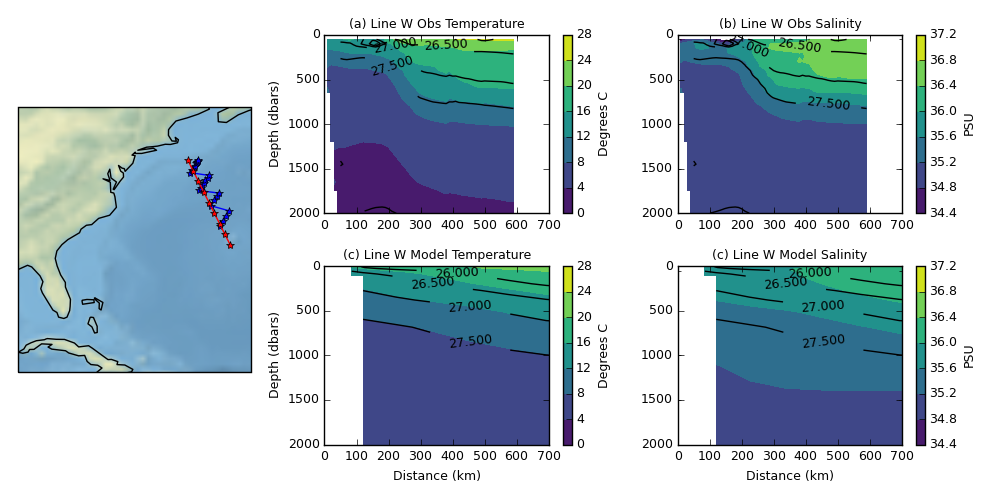
\includegraphics[width=\linewidth]{linew_interpolation.png}
\caption{Observational Line W and model interpolation. (a) and (b) climatologies of observational temperature and salinity. (c) and (d) Line W interpolated model temperature and salinity.}
\label{fig:observational_linew_model_interpolation}
\end{figure}

\subsubsection{Data Processing}
For purposes of visualization and comparison with the Earth System Model, the
data has been interpolated to a grid with a vertical resolution of 100 dbars and
horizontal resolution of 10 km. Cross-sections of oxygen concentration and mean
age (described below) for two years are shown in Figure~\ref{fig:obs_age_oxygen}.
Oxygen is generally high at the surface and decreases with depth, reaching a
minimum between depths 250 dbars and 750 dbars. Age on the other hand is at a
minimum at the surface and increases with depth. Figure~\ref{fig:obs_age_oxygen}
additionally shows the time-series of two locations along Line W (as indicated
by the black boxes). The first time-series (Figure~\ref{fig:obs_age_oxygen} (e))
suggests that there is a positive correlation between age and oxygen. The second
time-series (Figure~\ref{fig:obs_age_oxygen} (f)) on the other-hand shows the
anticipated negative relationship between age and oxygen.

Because temperature and salinity impact oxygen saturation, we additionally
compute the Apparent Oxygen Utilization for the observational data:

\begin{equation}
AOU = O_{2 sat} - O_2
\end{equation}

where $O_{2 sat}$ is the equilibrium saturation concentration of oxygen,
calculated as a function of temperature and salinity, and $O_2$ is the observed
oxygen concentration. The AOU is a measure of how under-saturated the oxygen sample
is. Using the AOU instead of oxygen concentration allows us to ignore the impacts
of temperature on the oxygen measurement.


\begin{figure}
\centering
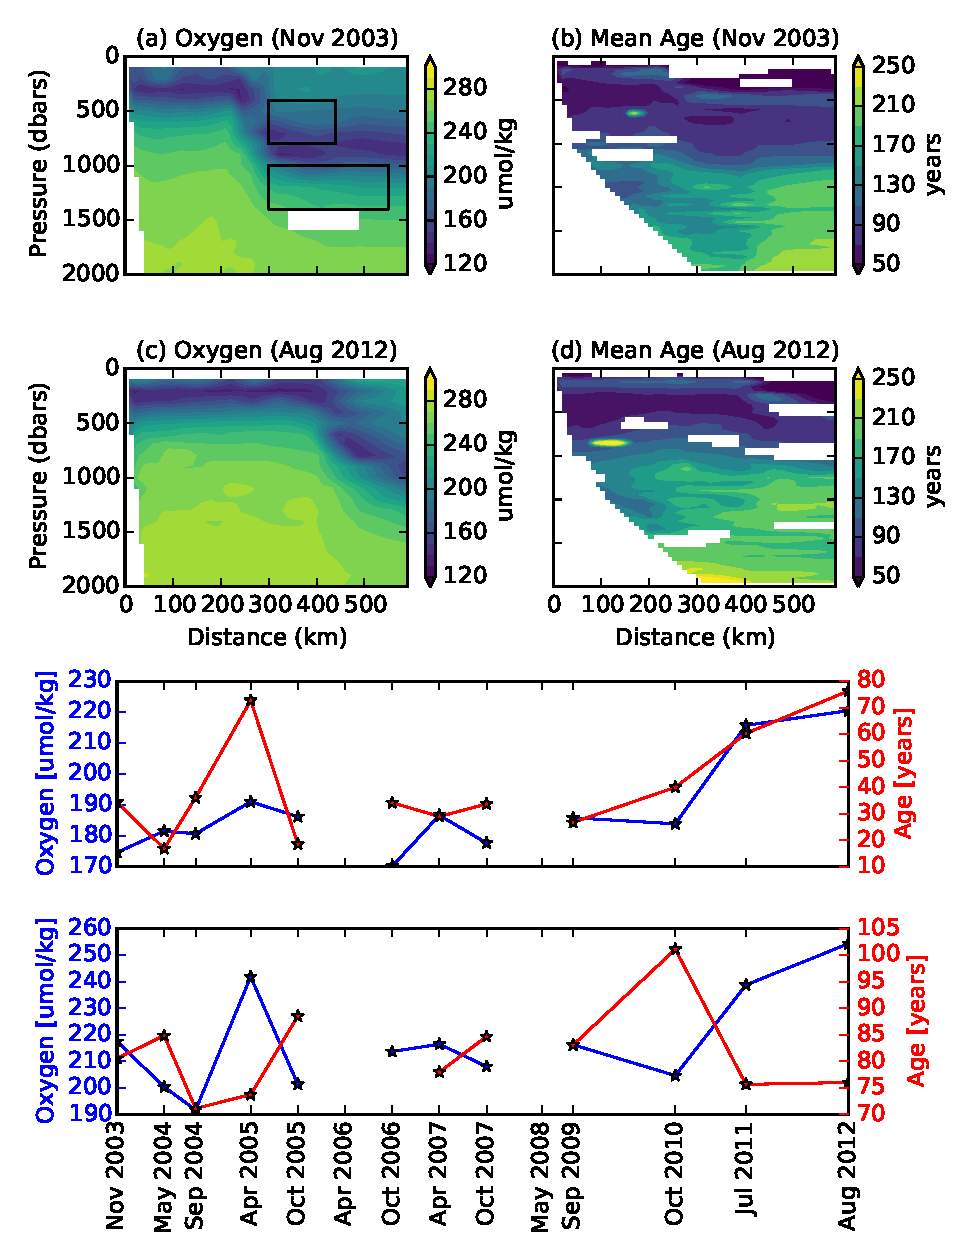
\includegraphics[width=\linewidth]{age_oxygen_ts.pdf}
\caption{Observational age and oxygen for two years. Subplots (a) and (b) show observational oxygen and
age from November 2003 while (c) and (d) show the oxygen and age from August 2012.
(e) and (f) show the timeseries of oxygen (blue) and age (red) averaged over the
boxes shown in subplot (a).}
\label{fig:obs_age_oxygen}
\end{figure}

\subsubsection{Mean Age Calculation}
A critical component to understanding ocean circulation and quantifying biological respiration is estimating the age of the water - or how long since the water was last in contact with the surface. Doing this with observations is not easy, but transient tracers make it possible. Because of the atmospheric time history of Chloroflourocarbons (CFCs), and the fact that CFCs have no sources and sinks in the ocean, CFCs are often used to quantify the age of ocean water. The simplest way of doing this is to assume that CFCs are in equilibrium with the atmosphere when they leave the ocean surface and are then transported advectively to the observation site. One can then deduce the date at which the water was subducted by matching the partial pressure of CFCs in the water to the date at which they had that concentration in the atmosphere.  This assumes that the transport to a given point can be characterized by a single timescale- the advective time.
In reality, estimating the age is complicated by mixing in the ocean. Because all flow is a combination of advective and diffusive flow, there is no one timescale that characterizes the time that a parcel of water has taken to reach an interior location from the surface. Because of this advective and diffusive flow, we characterize the timescales of a given point in the ocean interior with a distribution if transit times (or transit time distribution).
	The basis for this transit time distribution (TTD) approach for estimating ocean age is that for steady transport, the interior concentration of a transient tracer, $c(r,t)$, is given by (Haine and Hall, 2002):

\begin{equation}
	c(r,t) = \int_{0}^{\infty}c(t-t')G(r,t')dt'
\end{equation}

where $G(r,t)$ is a function describing the TTD at location r and time t. Measurements of CFC-12 were used to estimate the TTD assuming that (1) the TTD follows an Inverse Gaussian distribution and (2) the ratio of the mean width to mean age ($\Delta⁄\Gamma$) of the Inverse Gaussian is approximately equal to 1 (Waugh et al, 2003; Waugh et al, 2004; Waugh et al, 2006). Making the assumptions in order to estimate $G(r,t)$ using the Line W CFC-12 data and using the atmospheric history of CFC-12 allows us to estimate the mean age of the water sample.

\subsection{Model Simulation}
In addition to the observational data, we use an Earth system model (GFDL ESM2Mc)
to quantify the relationship between oxygen and age. GFDL ESM2Mc~\citep{Galbraith2011}
is a coarse resolution configuration of the GFDL ESM2M~\citep{Dunne2012}. The model
has an atmospheric resolution of 3.875$^{\circ}$ $\times$ 3$^{\circ}$  with 24 vertical levels. The ocean
model is non-Boussinesq, using pressure as the vertical coordinate, and has a
resolution of 3$^{\circ}$ $\times$ 1.5$^{\circ}$  and 28 vertical levels. The oceanic model also has a
coupled biogeochemical module referred to as the Biogeochemistry with Light Iron
Nutrients and Gases (BLING) model~\citep{Galbraith2010}. Although this module
uses a highly parameterized biological cycle, it predicts patterns of carbon and
oxygen change in response to global warming that are very similar to a more
complex biogeochemistry simulation in ESM2M~\citep{Small2014}. The model
also computes an ideal age~\citep{Thiele1990}, setting this tracer to
zero in the surface box and allowing it to increase at 1 yr/yr in the ocean
interior. For a full description of the model simulation, reference Section 3.2.1.

The model is interpolated to 1 $\times$ 1  grid in the North Atlantic and then
interpolated to a line extending from position (40$^{\circ}$N, 69$^{\circ}$W)
to (22$^{\circ}$N, 60$^{\circ}$W) to match observational Line W
(Figure~\ref{fig:observational_linew_model_interpolation} (a)). The model shows
a similar temperature and salinity profile on Line W compared with the
observations (Figure~\ref{fig:observational_linew_model_interpolation} (b) - (e)).
The model simulation is used to help put the observational analysis in in spatial
context and to investigate potential mechanisms affecting the age-oxygen relationship.

\begin{figure}
\centering
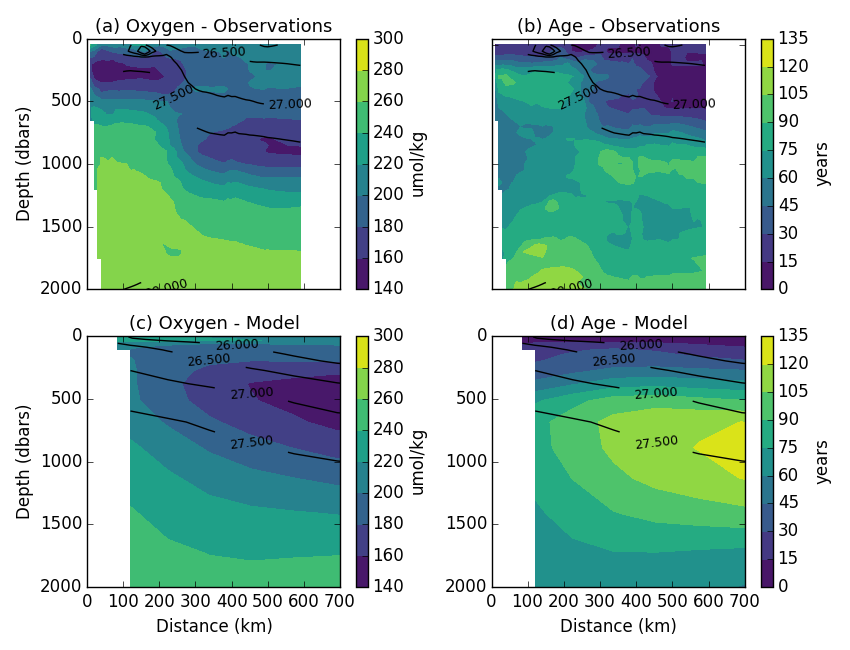
\includegraphics[width=\linewidth]{age_oxygen_climatology.png}
\caption{(a) Oxygen climatology and (b) age climatology from observations along Line W.
Contour lines show average neutral density. (c) Oxygen climatology and (d) age
climatology from the model simulation. Contour lines show the average netural density.}
\label{fig:oxygen_age_climatology}
\end{figure}

%%%%%%%%%%%%%%%%%%%%%%%%%%%%%%%%%%%%%%%%%%%%%%%%%%%%%%%%%%%%%%%%%%%%%%%%%%%%%%%%
% RESULTS
%%%%%%%%%%%%%%%%%%%%%%%%%%%%%%%%%%%%%%%%%%%%%%%%%%%%%%%%%%%%%%%%%%%%%%%%%%%%%%%%
%% Section 1
\section{Results}
\label{section:results}
\subsection{Age and Oxygen Relationship}

The climatologies of the calculated mean tracer age and oxygen concentration from
the Line W observations are shown in Figure~\ref{fig:oxygen_age_climatology} (a)
and (b). As expected, on large spatial scales there appears to be a negative relationship between the age and oxygen.
There is relatively high oxygen concentration and zero age at the surface, consistent
with the surface waters being in contact with the atmosphere, resulting in
near-equilibrium in oxygen and CFC concentrations. Age then generally increases
with depth, reaching a local maximum at just below the average depth of the 27.5
neutral density surface. Oxygen on the other hand generally decreases with depth,
reaching a local-minimum along the average depth of the 27.5 neutral density surface.
The spatial patterns of age and oxygen generally point towards a negative relationship
between the two qualities, particularly at intermediate depths. Oxygen shows a
core of minimum values with two intense patches, where the concentrations drop
below 160$\mu$mol kg$^{-1}$, on either side of the Gulf Stream more or less aligned
with the 27.5 neutral density surface. Age also shows two such patches of high
values on either side of the Gulf Stream at similar depths. However, there are
interesting differences in the detailed structure. First, the age maximum just
below the ventilated thermocline at distances 300-500 km offshore occurs at a depth of 1000
dbars. This is lower in the water column than the oxygen minimum, which occurs
at an approximate depth of 800 dbars. Additionally, there is significantly more
spatial variability in the age in the deeper regions across all distances than
is seen in the oxygen climatology. These differences between the spatial patterns
suggest the relationship between age and oxygen is likely more complicated than has
been suggested in previous work.

As discussed in the introduction, we also examine the age-oxygen relationship in
an Earth System Model. The vertical structure of the modeled oxygen and age
climatologies (Figure~\ref{fig:oxygen_age_climatology} (c) and (d)) are similar
to the observed climatologies, though somewhat offset in density space. The
modeled oxygen concentration exhibits a local minimum close to the 27.0 average
neutral density surfaces, while the age reaches a local maximum on the 27.5
average neutral density surface. While the vertical structure of age and oxygen
in the model are similar to the observations, there is a more obvious offset
between the depths of the local oxygen minimum and local age maximum in the model.
As with the observational data, this suggests a possible breakdown of the suggested
negative relationship between age and oxygen in this region. Note also that our
relatively coarse model does not allow for separation of two cores of low oxygen
water by the Gulf Stream-only the offshore core seen in the observations
is simulated with some measure of fidelity.

To better quantify the temporal relationship between mean age and oxygen, the
Pearson correlation coefficient between age and oxygen is calculated for
locations along Line W (Figure~\ref{fig:correlations} (a)).  Although this figure shows the anticipated
negative correlation between age and oxygen, in much of the plot the correlations
are relatively low.  Moreover, two regions of positive correlation are apparent
between 200 and 400 km offshore. One positive correlation region is at approximate
depths 500-750 dbars (between neutral density surfaces 27.0 and 27.5), and the
second is slightly deeper at depths 1250 - 2000 dbars.

One possible reason for the lack of a tight relationship between oxygen and age
is that oxygen concentration depends on solubility and thus on temperature and
salinity. In order to correct for this effect, we also examine the relationship
between the age and AOU. The AOU is a measure of how under-saturated the oxygen
concentration is. This under-saturation is usually due to the biological
consumption of oxygen but may also see an effect from incomplete equilibration
of sinking source waters, particularly in convective regions. Analyzing the
relationship between AOU and age gives us similar information to the age-oxygen
relationship, however, because we are subtracting the oxygen concentration from
the oxygen saturation, the AOU-age relationship will be the opposite sign
(mainly positive) and the AOU-age relationship removes the impacts of temperature
(and salinity) on oxygen saturation.

The Pearson correlation coefficient between age and AOU
(Figure~\ref{fig:correlations} (b)) shows a positive relationship between the
two quantities.  Similar to the pattern seen in the age-oxygen correlation
coefficients (Figure~\ref{fig:correlations} (a)), there are two regions with
anomalous correlation. One upper region of near-zero correlation, corresponds
with the upper region of positive correlation seen in Figure~\ref{fig:correlations}
(a). This suggests that this positive correlation between age and oxygen in this
region largely results from temperature effects. Younger waters in this region
are colder and thus hold more oxygen-countering any impacts from less
remineralization. Note however, that even with temperature effects removed the
AOU-age correlation remains low. Moreover, the region with anomalous O2-age
correlation in the deeper waters also shows an anomalous AOU-age correlation
(negative).  The fact that these patterns exist in the age-AOU correlation pattern
in addition to the age-O2 correlation pattern suggest that we need to find a
mechanism other than solubility changes for explaining such variability.

\begin{figure}
\centering
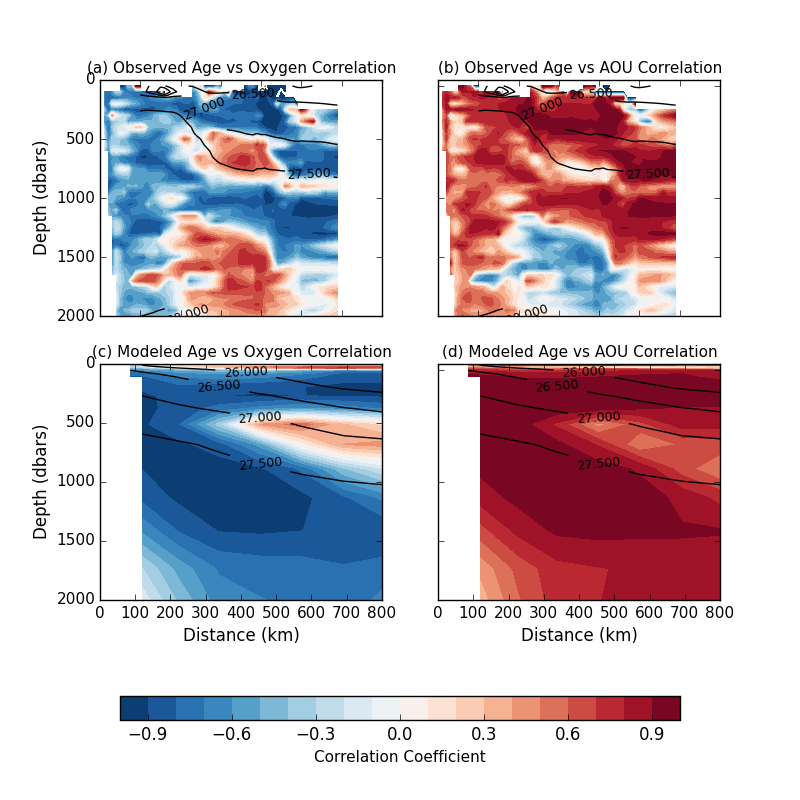
\includegraphics[width=\linewidth]{correlation.png}
\caption{Pearson correlation coefficients for age versus (left) oxygen and (right)
AOU for Line W observations. Contour lines indicate average neutral density climatology.}
\label{fig:correlations}
\end{figure}

We also show the Pearson correlation coefficient for the model simulation
(Figure~\ref{fig:correlations} (c) and (d)). Although the model also shows the
expected negative correlation between age and oxygen over much of the domain,
the correlation is far from uniform with one core of strong positive correlation
in denser waters around 1000 dbars and a second layer of negative correlation at
around 300 dbars.  As in the observations, there is a region of positive correlation
(with correlation coefficient of approximately 0.4) between the negative correlation
layers, starting at distance 400 km and extending to the end of Line W. This region
of positive correlation is similar to the upper region of positive correlation seen
in the observational record. Interestingly, in the model simulation, there is no
deeper region of positive correlation as seen in the observational correlation,
although there is a decline in the correlations as one approaches the coast below
1500 dbars.

The modeled age-AOU temporal correlation shows a very consistent pattern with the
modeled age-oxygen correlation. The area of anomalous correlation (now negative)
around depth 500 dbars is greatly reduced in Figure~\ref{fig:correlations} (d),
suggesting that a fraction of the positive correlation seen in the age-oxygen
correlation is due to solubility- a signal similar to that seen in the observations.
However, as in the observations this region still has a reduced positive correlation,
suggesting some additional mechanism is impacting the age-AOU relationship.

\subsection{Age and Oxygen/AOU Scatterplots}

To better visualize and analyze the relationship between the mean age and oxygen
along observational Line W, we show the scatter plot of age versus oxygen in
Figure~\ref{fig:scatter_plots} (a). The scatter points are colored with each
location's temporal correlation coefficient (same as in Figure~\ref{fig:correlations}
(a)). The ``S-shape'' of the age-oxygen scatterplot relationship roughly follows
the depth of the water column, with the surface waters at the left end of the
``S-shape'' and the deep waters at the right end. The positive correlation regions
indicated from Figure 4 (a) also appear in this relationship.

The scatter plot relationship between age and AOU is also shown
(Figure~\ref{fig:scatter_plots} (b)).  Similar to the age-oxygen scatter plot,
the age-AOU scatter plot also roughly follows depth, with the surface waters at
the left-hand side of the scatter plot, transitioning to the deeper waters at
the right hand-side. The upper region of reduced/zero correlation discussed in
Figure~\ref{fig:correlations} (b) is seen on this diagram at an age of 50 years,
just before the maximum in AOU. Additionally, the deeper region of negative
correlation discussed in Figure 4 (b) is seen on this diagram on the almost-flat
tail end of the scatterplot. Visualizing the age-AOU relationship in this way is
a powerful tool because it allows us to gain initial insight to the mechanisms
governing the AOU variability. The dashed lines represent expected linear
relationships between age and AOU with the slope of the linear relationship being
directly proportional to the rate of remineralization. At the surface, where
sinking particulate matter has higher concentrations and is more easily decomposed,
we have increased rates of remineralization, and therefore we would expect the
age-AOU relationship to follow one of the linear relationships with a higher slope.
As we move deeper in the water column, the slopes should decrease to reflect the
slower rates of remineralization in the deep ocean.

If the variability in AOU were driven exclusively by changes in the rate of
ventilation (but not the pathways of ventilation or the rate of remineralization),
we would expect the age-AOU relationship to fall along one of the dashed lines.
The upper region does follow this linear relationship (with a slope of
1.7$\mu$mol yr$^{-1}$). When the age-AOU relationship does not follow these linear
lines however, it indicates that other processes are influencing the spatial
(and thus potentially the temporal) variability in AOU. The right-hand tail of
this relationship, where the correlation is negative, does not follow the
anticipated linear relationship, and therefore we can infer that some additional
process is influencing the AOU-age relationship. This region is also one where
the correlation between AOU and age is (unexpectedly) negative.

The shape of the modeled relationship between age and oxygen is similar to the
shape of the observed age-oxygen relationship (Figure~\ref{fig:scatter_plots} (a)),
suggesting that the model captures the mean relationships to a surprising extent
(given the coarseness of its resolution and the simplicity of its biological model).
However, there are clear differences between the modelled and observed variability.
In the model, the area of positive correlation between the age and oxygen occurs
in the region of the oxygen minimum, which is a region where the age is still
increasing with depth. Since the shape of the relationship roughly follows depth,
movement along this curve would correspond to vertical movement in the water column.
In this region, if we move lower in the water column, age increases and oxygen also
increases, therefore resulting in a positive correlation. This suggests that vertical
movement in the water column could be causing the positive correlation. In the
observations, however, the upper region of positive correlation is found above the
oxygen minimum and the lower region is found around a weak age minimum. The
corresponding point on the modelled age-oxygen plot shows some near-zero correlations,
but no positive values.

\begin{figure}
\centering
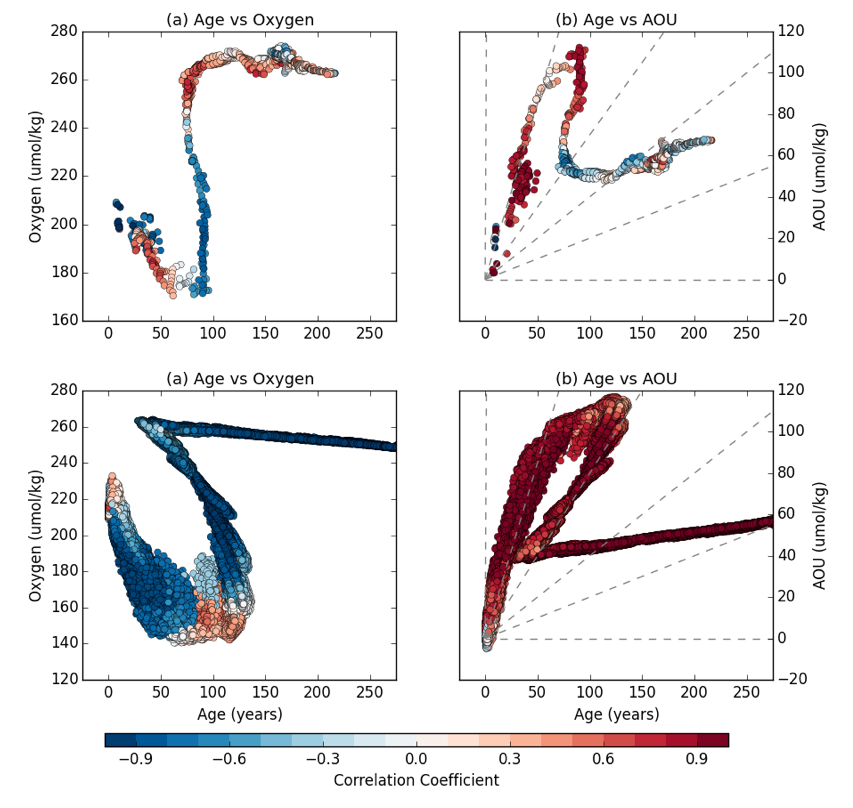
\includegraphics[width=\linewidth]{age_aou_scatter.png}
\caption{Scatter plot of age versus observed (a) oxygen and (b) AOU and
modeled (c) oxygen and (d) age for distances 300-400 km.
Colors indicate correlation coefficient of given relationship. Dashed grey lines indicate linear relationship between age and AOU.}
\label{fig:scatter_plots}
\end{figure}

The modeled age-AOU scatter plot (Figure~\ref{fig:scatter_plots} (d)) has
similarities to the observed age-AOU relationship (Figure~\ref{fig:scatter_plots}
(b)), but has a much more pronounced mid-depth age minimum. As in
Figure~\ref{fig:scatter_plots} (b), the dashed grey lines represent the linear
relationship between the age and AOU. In the upper region of the domain, the age
and AOU follow this linear relationship quite closely (with a slope of 1.7$\mu$mol yr$^{-1}$
- similar to the observations). Slightly deeper in the water column, the age and
AOU also closely follow a linear line, with a slightly smaller slope (slope of 0.8).
In the deeper waters however, the age-AOU relationships break away from the linear
model, suggesting additional processes impacting the AOU variability.

Some part of the mean relationship is driven by the well-known decrease in the
remineralization of organic material with depth~\citep{Armstrong2002,Klaas2002}
as unprotected organic materials are preferentially consumed near the surface.
This would move points between a steeply-sloped linear relationship near the
surface to lying along a line with a flatter slope at depth. An additional
factor is that the pathways of ventilation change with depth, with waters near
the deep age minima more affected by the southward flow of North Atlantic Deep
Water. These different factors have the potential to affect the variability as
well. In particular, changing pathways of ventilation would be expected to
change the mix of water masses seen at a given point. Assuming the water masses
involved in this mixing are reflected in the AOU-age structure, such changes
might be expected to produce relationships parallel to the age-AOU curve - which
in many locations would imply anti-correlation (where the mean curve slopes down
to the right) or near-zero correlation (where the mean curve is oriented either
horizontally or vertically). We note that when the age-AOU curve lies along one
of these dashed lines, it is impossible to distinguish changes in ventilation
rate from changes in water mass type without bringing in more information.

The region of reduced positive correlation seen in the depth profile of the age-AOU
Pearson correlation coefficient (Figure~\ref{fig:correlations} (d)) is seen in the
age-AOU scatterplot (Figure~\ref{fig:scatter_plots} (d)) at the apex of the scatter
plot, where the AOU goes from increasing with age to decreasing with age. This
region occurs between the two regions of strong linear relationship between age
and AOU as discussed above. This result suggests that it is a change in the
fraction of water associated with two water masses that is contributing to the
reduced positive correlation in age versus AOU (or positive in the age-oxygen
correlation).

This analysis provides some initial insight to why the age-oxygen relationship
displays an area of positive correlation. The age-AOU scatter plot suggests that
mixing between water masses may be contributing to the anomalous correlation in
the age-oxygen and age-AOU relationships. In the next section, we will investigate
the mechanisms driving the modeled variability in age and oxygen further,
examining whether the results can be simply explained in terms of vertical
excursions of density, or whether more subtle changes in circulation are involved.

\subsection{Mechanisms Driving Age and Oxygen Variability}
In this section, we will use the model simulation to assess the spatial extent of
the anomalous correlation outside of Line W and diagnose the most likely mechanisms
responsible for the break-down in the anticipated age-AOU relationship.

\subsubsection{Horizontal Extent of Anomalous Correlation}

To determine the horizontal extent of the anomalous correlation between age and
AOU, we show the age-AOU temporal correlation from the model on various neutral
density surfaces over the entire North Atlantic basin (see left-hand side of
Figure~\ref{fig:iso_correlations}). These correlations show that the temporal
relationship between age and AOU is largely positive throughout the entire domain
with Pearson correlation coefficients exceeding 0.6 in most of the basin. There
is a region at the end of Line W where the age-AOU correlation is reduced. This
is most prominently seen on the lower neutral density surfaces
(Figures~\ref{fig:iso_correlations} (e) and (g)).

The subplots on the right-hand side show the correlation on each designated
density surface ignoring the impacts of vertical heave in the isopycnals, while
the subplots on the left side do include vertical isopycnal heave as described
by the following equations:

\begin{equation}
	r_{\mathrm{with \; heave}} = \mathrm{corr}(\Gamma, O_2)|_{\gamma_n = 27.0}
\end{equation}

\begin{equation}
	r_{\mathrm{without \; heave}} = \mathrm{corr}(\Gamma|_{\gamma_n = 27.0}, O_2|_{\gamma_n = 27.0})
\end{equation}

In both equations (4.4) and (4.5) above, $\gamma_n$ designates the depth of a
neutral density surface and the overbar designates the time average. It is
important to distinguish between these two methods of neutral density interpolation
because the 'with heave' method includes the impact of vertical motion and allows
us to determine the extent that vertical motion impacts the correlation. The
positive correlation appears to be more significantly reduced on the neutral density
surfaces including vertical heave (left-hand side subplots). These results
suggest that the mechanism decoupling age and AOU is spatially limited to the
region at the end of Line W and includes some component of vertical mixing.

\begin{figure}
\centering
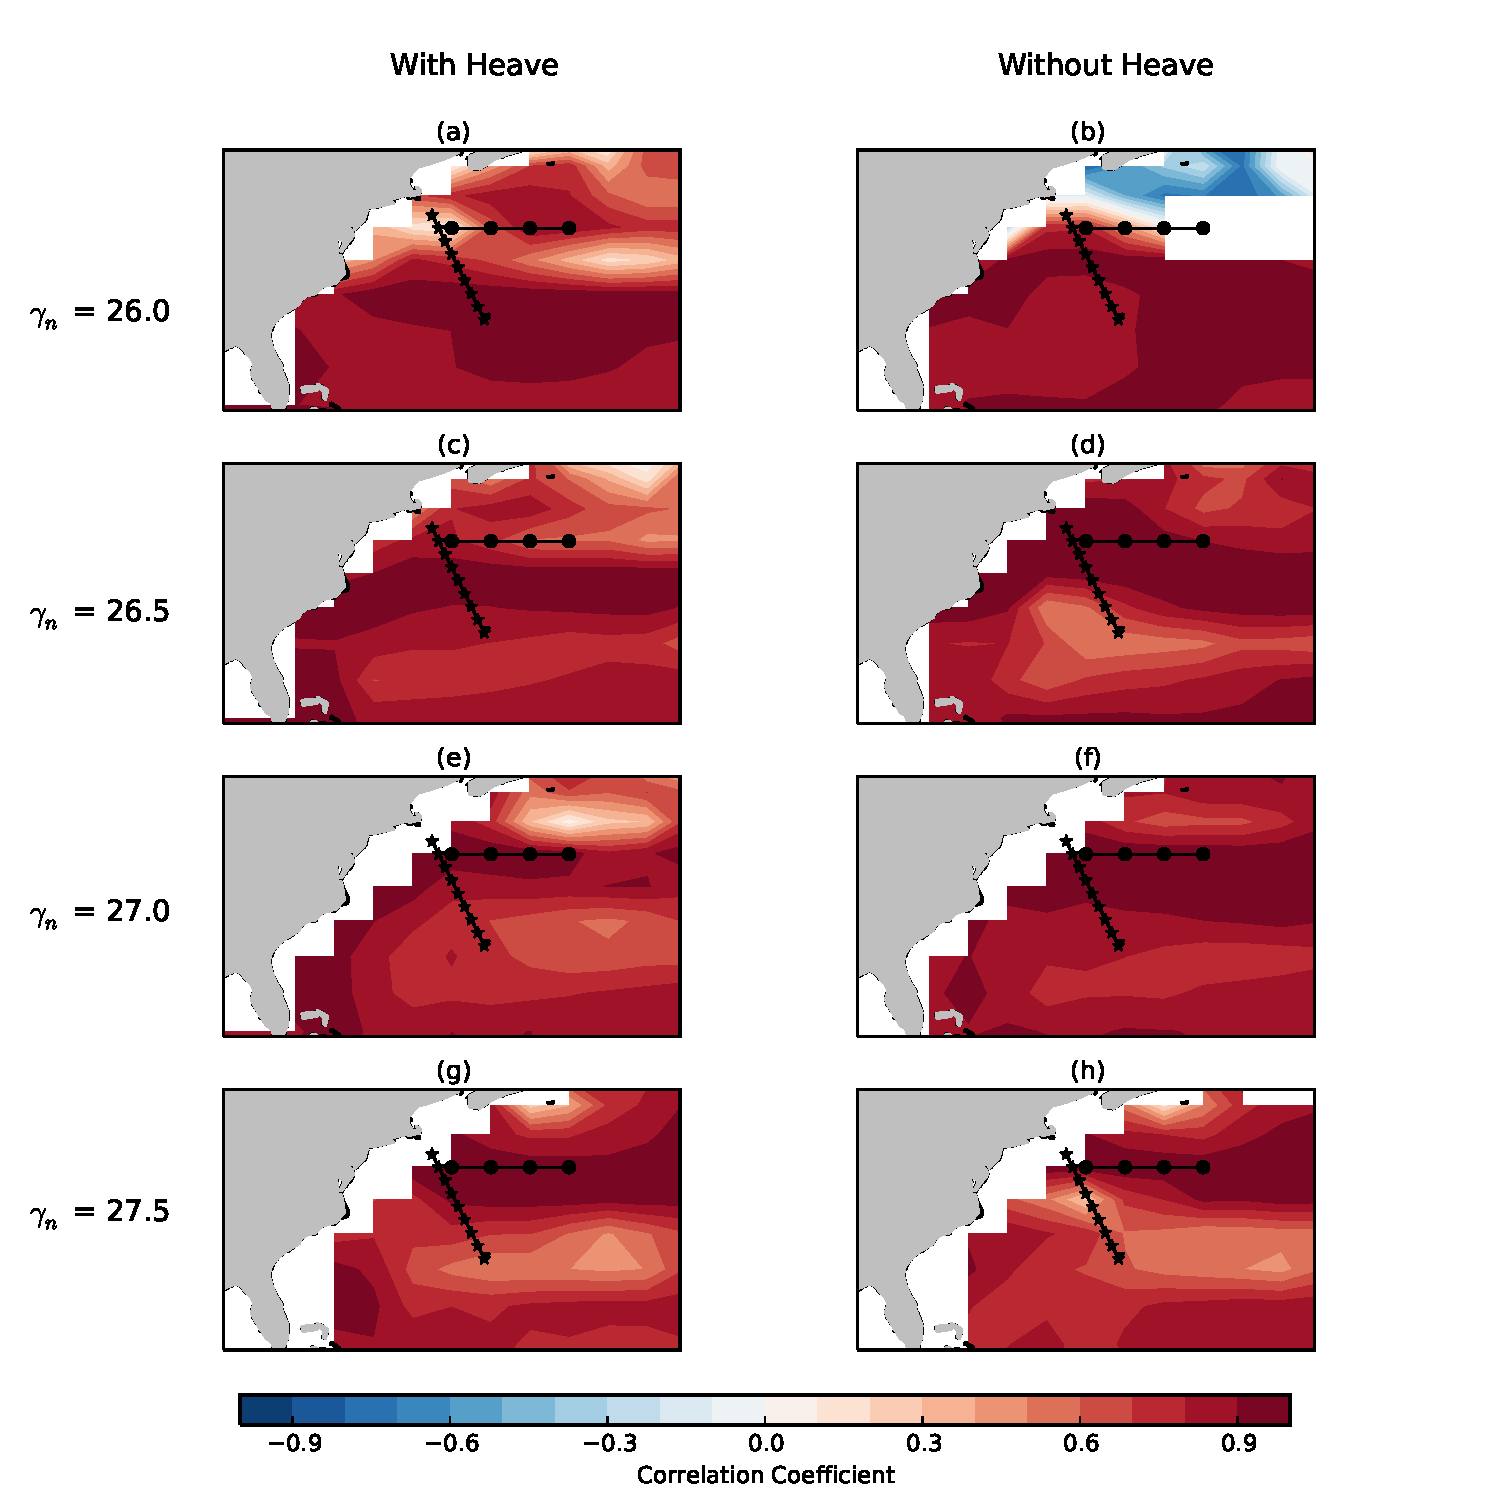
\includegraphics[width=\linewidth]{age_aou_corr_iso_sfc.pdf}
\caption{Correlation between age and AOU on various isopycnal surfaces. Left column indicate correlation calculated on average depth of the isopycnal surface, and therefore including contributions from isopycnal heave. Right column shows correlation calculated on the isopycnal surface and does not include contributions from heave.}
\label{fig:iso_correlations}
\end{figure}

\subsubsection{Line W versus Line 40N}
In order to diagnose what is causing this reduction in the negative age-oxygen
correlation and positive age-AOU correlation, we examine a region of the North
Atlantic where this breakdown of the age-AOU relationship does not occur and compare
it with Line W. We refer to this region as Line 40N, a hypothetical transect that
extends from Cape Cod eastward along latitude line 40 N. This hypothetical
transect follows along a region of the North Atlantic basin where the age-oxygen
correlation is strongly negative (not shown) and the age-AOU correlation is
strongly positive for all neutral density surfaces (Figure~\ref{fig:iso_correlations}).
Comparing Line 40N and Line W allows us to evaluate the differences between the
two and understand why Line W experiences these low correlations in the age-AOU
relationship.

One possible reason Line 40N maintains a strong positive correlation is due to
strong horizontal (primarily along-isopycnal) variability relative to Line W.
In order to diagnose the relative contributions of this along-isopycnal
variability and the isopycnal heave variability, we break the time rate of change
of age and AOU as follows:

\begin{figure}
\centering
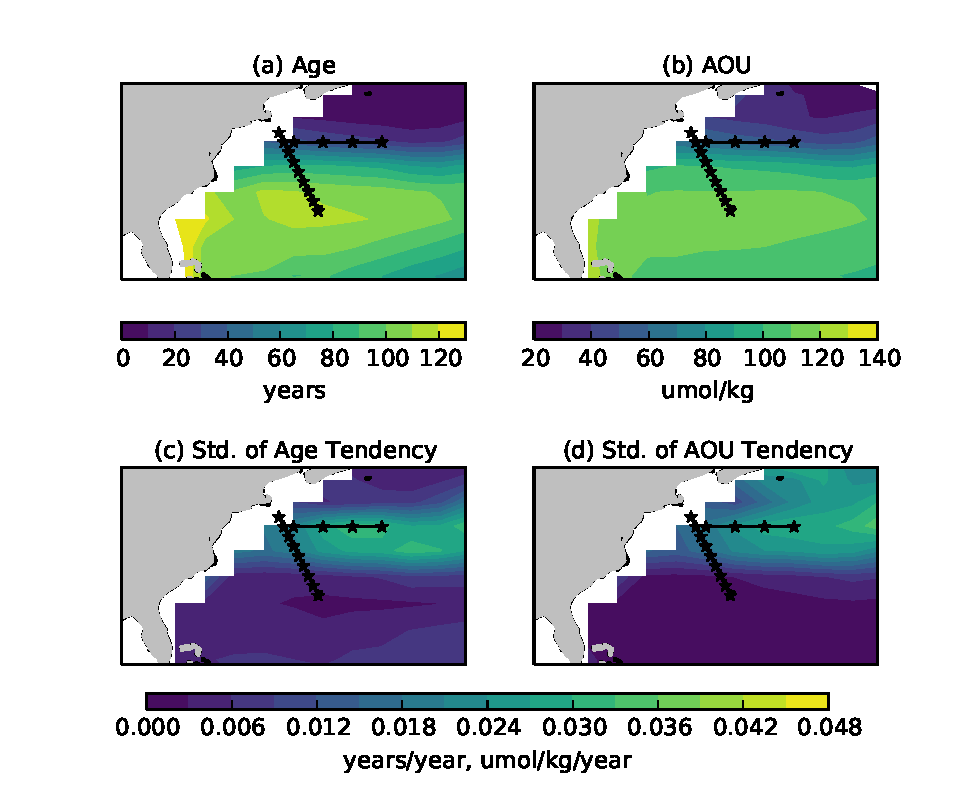
\includegraphics[width=\linewidth]{spice_figure.pdf}
\caption{Climatologies of (a) age and (b) AOU interpolated on neutral density surface 27.0. Bottom: Standard deviation of (c) age tendency and (d) AOU tendency interpolated on neutral density surface 27.0. Bottom plots are calculated as the standard deviation of the first term on right-hand side of equation (4).}
\label{fig:spice}
\end{figure}

\begin{equation}
	\left. \frac{\mathrm{d}\Gamma}{\mathrm{d}t}\right|_z = \left. \frac{\mathrm{d}\Gamma}{\mathrm{d}t}\right|_{\gamma_n=27.0} + \left. \frac{\mathrm{d}z}{\mathrm{d}t}\right|_{\gamma_n=27.0} \frac{\mathrm{d}\Gamma}{\mathrm{d}z}
\end{equation}

\begin{equation}
 \left. \frac{\mathrm{d}AOU}{\mathrm{d}t}\right|_z = \left. \frac{\mathrm{d}AOU}{\mathrm{d}t}\right|_{\gamma_n=27.0} + \left. \frac{\mathrm{d}z}{\mathrm{d}t}\right|_{\gamma_n=27.0} \frac{\mathrm{d}AOU}{\mathrm{d}z}
\end{equation}

\begin{figure}
\centering
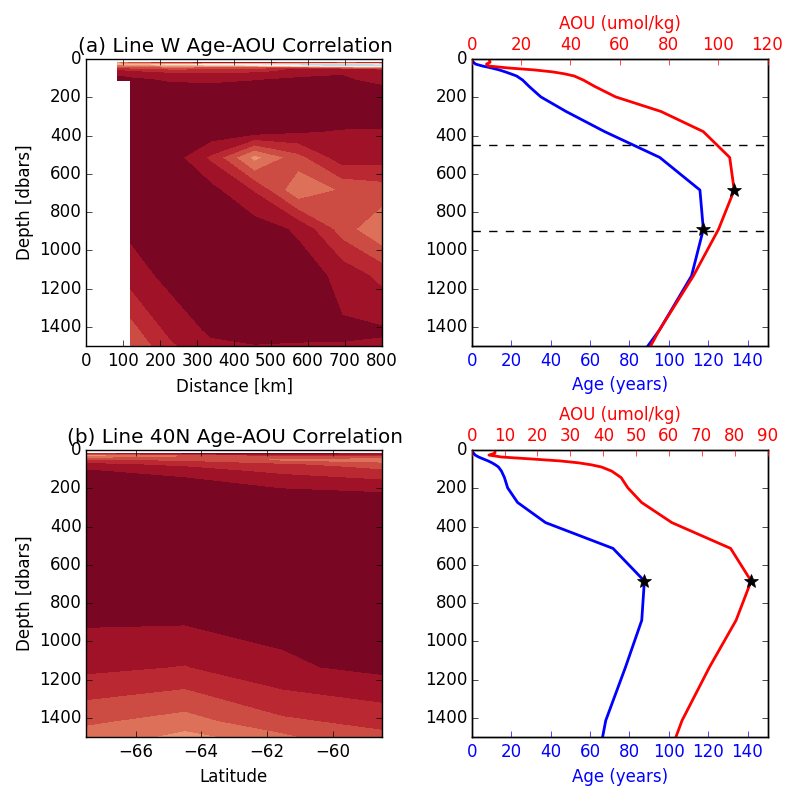
\includegraphics[width=\linewidth]{age_aou_corr_linew_line40N.png}
\caption{Age-AOU correlation and vertical profiles for (top) Line W and (bottom) Line 40N.}
\label{fig:vertical_profile}
\end{figure}

where the first term on the right-hand side refers to the age tendency on the
neutral density surface and the second term on the right-hand refers to the
contribution of vertical heave to the age variability. The climatologies of age
and oxygen on the $\gamma_n$=27.0 surface along with the standard deviation of the age
and oxygen tendencies along this surface are shown in Figure~\ref{fig:spice}.
The end of Line W, where the age-AOU correlation is near zero, lies in a
region where there is reduced horizontal gradient in age and oxygen. This is
significantly different to Line 40N, which lies in a region where the horizontal
gradients in age and oxygen (primarily in the meridional direction) are
particularly strong. This results in significantly more along-isopycnal variability
along Line 40N than Line W, as shown in figure~\ref{fig:spice} (c) and (d).
Because of the reduced along-isopycnal variability on Line W, the vertical heave
component (second term on right hand side of equations 4.6 and 4.6) may be important
in setting up the reduced positive correlation between age and AOU.

To investigate the vertical heave contribution to the age-AOU correlation, we show
the correlation between age and AOU for Line W and Line 40N in Figure~\ref{fig:vertical_profile}.
As previously discussed, Line W has an anomalous region of near-zero correlation.
Line 40N on the other hand has a strong positive correlation between age and AOU
in the upper 1500 dbars of the cross section. Figure 8 also compares the vertical
profiles of age and AOU along both lines. There is a visible offset between the
depths of the age and AOU maximum (as indicated by the stars) with the age
maximum occurring lower in the water column (900 dbars) than the AOU maximum
(700 dbars). Between the age and AOU maximums, age increases with depth and AOU
decreases with depth. It is between these depths that the reduced positive
correlation occurs between age and AOU (as indicated by dashed lines in
Figure~\ref{fig:vertical_profile}). We propose that the reduced correlation occurs
because of vertical motion acting on this particular vertical gradient in age and
AOU. When comparing the vertical profiles on Line W with Line 40N, we see that
there is no offset between the age and AOU maximums on Line 40N. We also examined
the magnitude of the vertical motion of the isopycnal surfaces (not shown) and
found no significant difference between Line W and Line 40N. While both transects
have similar levels vertical motion, the presence of a depth offset between the age
and AOU maximum in addition to decreased along-isopycnal variability result in
Line W having a reduced correlation between age and AOU.

Line W is unusual because the along-isopycnal (horizontal) gradients are so small
that variations in mixing or along-isopcynal velocity will have relatively small
impacts. This allows the vertical heave to dominate the local
variability in age and oxygen. Between depths 500 dbars - 750 dbars, this vertical
heave acts on an offset in the depths of the age maximum and oxygen minimum,
resulting in the observed positive correlation. In other regions of the basin
(Line 40N), the horizontal variation in transport is large enough to dominate the local variability.
Even though the same vertical heave and age maximum and oxygen minimum depth
offset is seen in this region, the large magnitude of horizontal variability maintains
the expected age-oxygen relationship.


%%%%%%%%%%%%%%%%%%%%%%%%%%%%%%%%%%%%%%%%%%%%%%%%%%%%%%%%%%%%%%%%%%%%%%%%%%%%%%%%
% CONCLUSIONS
%%%%%%%%%%%%%%%%%%%%%%%%%%%%%%%%%%%%%%%%%%%%%%%%%%%%%%%%%%%%%%%%%%%%%%%%%%%%%%%%

\section{Conclusions}
\label{section:conclusions}

Our analysis of the Line W observations of age and oxygen show that there is a
much more complicated relationship between the two quantities than one would naively
expect. The commonly held expectation of a negative relationship between age and
oxygen breaks down along observational Line W due to two regions of positive correlation.
One region of positive correlation is seen within the ventilated thermocline and
the other is lower in the water column. The same upper region of positive correlation
is seen in an Earth System Model (GFDL ESM2Mc) representation of Line W. We
additionally remove the impacts of temperature on oxygen saturation, by looking
at the age correlation with AOU. The age-AOU correlation also shows anomalous
(zero to negative) correlation in the observational data set and model simulation.

\begin{figure}
\centering
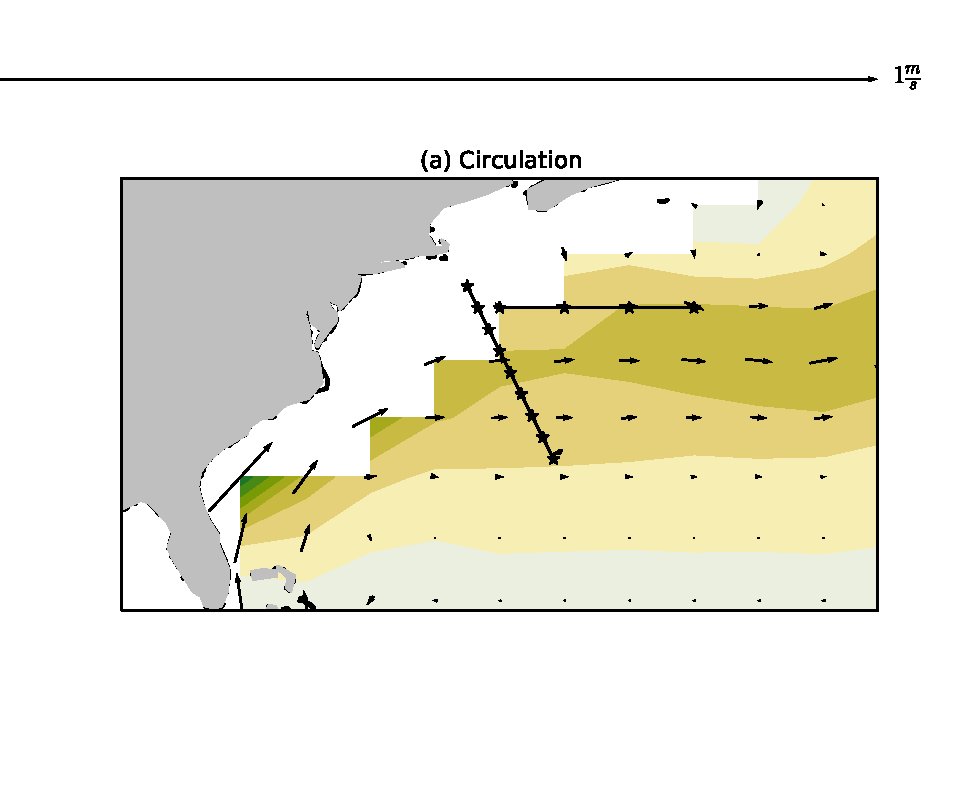
\includegraphics[width=\linewidth]{circulation.pdf}
\caption{Circulation on neutral density surface 27.0}
\label{fig:circulation}
\end{figure}

Our analysis of the Line W observations of age and AOU show that there is a much
more complicated relationship between the two quantities than one would naively
expect. The commonly held expectation of a positive relationship between age and
oxygen breaks down along observational Line W in two regions. One region of low
correlation is seen within the ventilated thermocline and the other is lower in
the water column. The same upper region of near-zero correlation is seen in an Earth
System Model (GFDL ESM2Mc) representation of Line W.

Because of the limited temporal resolution and spatial extent of the observational
data, we use the GFDL ESM2Mc to investigate the potential mechanisms causing the
anomalous correlation between and AOU. We show that the region of anomalous
correlation is limited to a region at the end of Line W, and to a few isopycnal
surfaces (surfaces 27.0-27.5). The end of Line W lies in a unique region in the
North Atlantic basin where the horizontal gradients in age and AOU are relatively
weak and thus the along-isopycnal variability is very small. Additionally, at the
bottom of the ventilated thermocline, there is a depth offset between the age
maximum and AOU maximum. Any vertical motion within this region, coupled with the
limited horizontal variability, would cause a break-down of the correlation between
the age and AOU.

The end of Line W is unique because it lies in the approximate center of the North
Atlantic gyre circulation (Figure~\ref{fig:circulation}). Because the horizontal
circulation in the middle of the gyre is very small, there is little horizontal
gradients in ocean tracers. In such regions, the balance between vertical heaving
of isopycnals (which acts to reduce age-AOU correlation) and horizontal mixing
(which mostly strengthens age-oxygen relationship) determines whether or not the
expected age-AOU relationship holds. Because of this delicate balance, one needs
to consider the local dynamics before assuming that oxygen and age follow a strong
negative relationship.



%\bibliography{/RESEARCH/library}
%%% Local Variables:
%%% mode: latex
%%% TeX-master: "thesis"
%%% End:
